\documentclass{standalone}

\usepackage{pgfplots} %%%%%% Regression %%%%
\pgfplotsset{compat = newest}
\usepackage{pgfplotstable}
\usepackage{tikz}
\usepackage{tikz-3dplot} %%%%%% Draw %%%%%%
\usepackage{tikz,tkz-euclide}
\usetikzlibrary{arrows,calc,patterns}
\usetikzlibrary{quotes,angles}
\usetikzlibrary{shapes.geometric}
\usepackage{circuitikz} %%%%% Circuit %%%%
\usetikzlibrary{decorations.pathmorphing,patterns}

\setlength{\unitlength}{1cm}
\usepackage[OT1]{fontenc}
\renewcommand*\familydefault{\sfdefault}
\usepackage{helvet,sfmath}
\begin{document}



\tikzset{every picture/.style={line width=0.75pt}} %set default line width to 0.75pt        

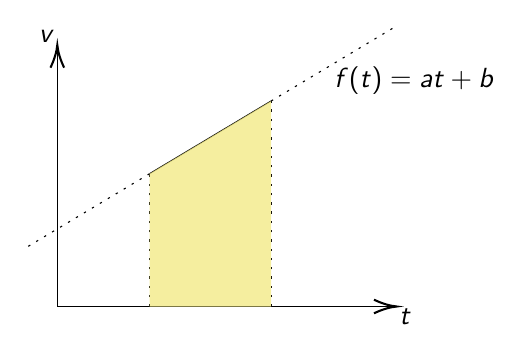
\begin{tikzpicture}[x=0.75pt,y=0.75pt,yscale=-1,xscale=1]
%uncomment if require: \path (0,15225); %set diagram left start at 0, and has height of 15225

%Straight Lines [id:da8478146938436368] 
\draw    (708,5561) -- (869.5,5561) ;
\draw [shift={(871.5,5561)}, rotate = 180] [color={rgb, 255:red, 0; green, 0; blue, 0 }  ][line width=0.75]    (10.93,-3.29) .. controls (6.95,-1.4) and (3.31,-0.3) .. (0,0) .. controls (3.31,0.3) and (6.95,1.4) .. (10.93,3.29)   ;
%Straight Lines [id:da426961800916945] 
\draw    (708,5561) -- (708,5437) ;
\draw [shift={(708,5435)}, rotate = 90] [color={rgb, 255:red, 0; green, 0; blue, 0 }  ][line width=0.75]    (10.93,-3.29) .. controls (6.95,-1.4) and (3.31,-0.3) .. (0,0) .. controls (3.31,0.3) and (6.95,1.4) .. (10.93,3.29)   ;
%Straight Lines [id:da9265838630395075] 
\draw    (752.5,5497) -- (811,5462) ;
%Straight Lines [id:da9378719035022547] 
\draw  [dash pattern={on 0.84pt off 2.51pt}]  (694,5532) -- (752.5,5497) ;
%Straight Lines [id:da4743725488552838] 
\draw  [dash pattern={on 0.84pt off 2.51pt}]  (811,5462) -- (869.5,5427) ;
%Straight Lines [id:da8191317525330123] 
\draw  [dash pattern={on 0.84pt off 2.51pt}]  (752.5,5561) -- (752.5,5497) ;
%Straight Lines [id:da9554702110291705] 
\draw  [dash pattern={on 0.84pt off 2.51pt}]  (811,5561) -- (811,5462) ;
%Shape: Polygon [id:ds6962765470590839] 
\draw  [draw opacity=0][fill={rgb, 255:red, 242; green, 234; blue, 133 }  ,fill opacity=0.79 ] (752.5,5497) -- (811,5462) -- (811,5561) -- (752.5,5561) -- cycle ;

% Text Node
\draw (708,5435) node [anchor=south east] [inner sep=0.75pt]    {$v$};
% Text Node
\draw (871.5,5561) node [anchor=north west][inner sep=0.75pt]    {$t$};
% Text Node
\draw (840.25,5444.5) node [anchor=north west][inner sep=0.75pt]    {$f( t) =at+b$};


\end{tikzpicture}
\end{document}